\documentclass[UTF8,fontset=windows]{ctexart}
\usepackage[a4paper,margin=22mm]{geometry}
\usepackage{amsmath,amssymb}
\usepackage{tikz}
\usepackage{booktabs}
\usepackage{enumitem}
\usepackage{xcolor}
\usepackage{float}
\usetikzlibrary{arrows.meta,calc,patterns}

\setlength{\parindent}{0pt}
\setlength{\parskip}{6pt}
\setlist[itemize]{leftmargin=2em,itemsep=2pt,topsep=2pt}

\definecolor{accent}{RGB}{32,92,148}
\definecolor{softblue}{RGB}{224,238,250}
\definecolor{softred}{RGB}{252,230,226}
\definecolor{axisgray}{RGB}{80,80,80}

\newcommand{\diff}{\,\mathrm{d}}

\title{\vspace{-1.5cm}\textbf{清华大学 2024 年《材料力学》（冯雪班）期末考试大题标准解答}}
\author{回忆整理版标准解答}
\date{}

\begin{document}
\maketitle
\vspace{-1.0cm}

\section*{一、空间折杆强度设计题（3D 弯扭组合）}

\textbf{1、图示空间折杆，圆截面直径为 $d$。AB 段位于 $x$ 轴上，长度为 $L$，A 端为固定约束，且 AB 承受向下（$-z$ 方向）的均布载荷 $q$；BC 段位于水平 $x-y$ 面内（平行于 $y$ 轴），长度为 $L$。C 端受垂直力 $F_z$ 和关于 $x$ 轴的集中弯矩 $M_x$，材料许用应力为 $[\sigma]$。求折杆的危险截面，并按第三强度理论进行强度校核。}

\begin{center}
\begin{tikzpicture}[scale=1.5, >=Stealth, x={(-0.35cm,-0.35cm)}, y={(1cm,0cm)}, z={(0cm,1cm)}]
    % Coordinate axes
    \draw[axisgray, ->] (0,0,0) -- (2.5,0,0) node[right] {$x$};
    \draw[axisgray, ->] (0,0,0) -- (0,2.5,0) node[above] {$y$};
    \draw[axisgray, ->] (0,0,0) -- (0,0,2.5) node[above] {$z$};
    
    % Draw beam segment AB
    \draw[ultra thick, accent] (0,0,0) -- (1.5,0,0);
    \node at (0,-0.2,0.2) {A (固支)};
    
    % Draw beam segment BC
    \draw[ultra thick, accent] (1.5,0,0) -- (1.5,1.5,0);
    \node[above] at (1.5,0,0.2) {B};
    \node[right] at (1.5,1.5,0) {C};
    
    % Distributed load on AB (along -z)
    \foreach \x in {0.2,0.5,0.8,1.1,1.4} {
        \draw[->, blue, thin] (\x,0,0.4) -- (\x,0,0.05);
    }
    \draw[blue, thin] (0.2,0,0.4) -- (1.4,0,0.4);
    \node[blue, above] at (0.8,0,0.4) {$q$};
    
    % Force Fz at C
    \draw[->, red, very thick] (1.5,1.5,0.6) -- node[right] {$F_z$} (1.5,1.5,0.05);
    
    % Moment Mx at C
    \draw[->, red, thick] (1.5,1.7,0) arc (90:360:0.2);
    \node[red, right] at (1.5,1.8,0) {$M_x$};
\end{tikzpicture}
\end{center}

\subsubsection*{解答：}

\textbf{（1）计算各截面内力}

截面为圆截面，弯曲截面系数 $W = \frac{\pi d^3}{32}$，极惯性矩截面系数 $W_p = \frac{\pi d^3}{16} = 2W$。
\begin{itemize}
    \item \textbf{BC 段}（$y$ 坐标自 0 到 $L$）：
    截面受 $F_z$ 引起的绕 $x$ 轴弯矩 $M_x(s) = F_z \cdot s + M_x$。无扭矩。
    最大弯矩在 B 点处：$M_B = F_z L + M_x$。
    \item \textbf{AB 段}（$x$ 坐标自 0 到 $L$）：
    外力对 AB 段任意截面 $x$ 的力矩效应为：
    \begin{itemize}
        \item 集中载荷 $F_z$ 产生绕 $y$ 轴弯矩：$M_y = F_z (L - x)$；产生绕 $x$ 轴的扭矩 $T = F_z \cdot L$。
        \item 均布载荷 $q$ 产生绕 $y$ 轴弯矩：$M_{y, q} = \frac{1}{2}q(L - x)^2$。
        \item C 端集中弯矩 $M_x$ 产生绕 $x$ 轴扭矩 $T_0 = M_x$。
    \end{itemize}
    综上，AB 段任意截面 $x$ 处的内力为：
    \[
        M_y(x) = F_z(L - x) + \frac{1}{2}q(L - x)^2
    \]
    \[
        T(x) = F_z L + M_x
    \]
\end{itemize}

\textbf{（2）危险截面分析}

内力在固定端 A 处 ($x = 0$) 达到最大值：
\[
    M_A = F_z L + \frac{1}{2}q L^2, \quad T_A = F_z L + M_x
\]
此即为整个折杆的\textbf{危险截面}。

\textbf{（3）强度校核（第三强度理论）}

圆截面弯扭组合，等效弯矩为：
\[
    M_{r3} = \sqrt{M_A^2 + T_A^2} = \sqrt{\left(F_z L + \frac{1}{2}q L^2\right)^2 + (F_z L + M_x)^2}
\]
最大当量应力为：
\[
    \sigma_{r3} = \frac{M_{r3}}{W} = \frac{32 \sqrt{\left(F_z L + \frac{1}{2}q L^2\right)^2 + (F_z L + M_x)^2}}{\pi d^3}
\]
校核强度准则：$\sigma_{r3} \le [\sigma]$。

\newpage

\section*{二、图乘法求复合梁中点挠度}

\textbf{2、简支梁总跨度为 $4L$，左、右两段长度为 $L$，弯曲刚度为 $2EI$；中间段长度为 $2L$，弯曲刚度为 $EI$。在中间段上作用向下均布载荷 $q$，试利用图乘法求梁中点的挠度。}

\begin{center}
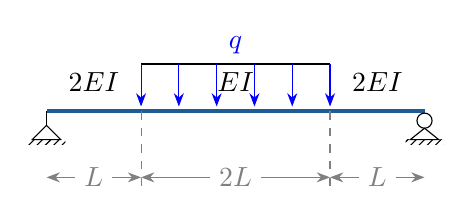
\begin{tikzpicture}[scale=1.2, >=Stealth]
    % Draw beam
    \draw[ultra thick, accent] (0,0) -- (4,0);
    
    % Draw supports
    \draw (0,-0.15) -- (0,0);
    \draw (0,-0.15) -- (-0.15,-0.3) -- (0.15,-0.3) -- cycle;
    \pattern[pattern=north east lines] (-0.2,-0.35) rectangle (0.2,-0.3);
    
    \draw (4,-0.1) circle (0.08);
    \draw (4,-0.18) -- (3.85,-0.3) -- (4.15,-0.3) -- cycle;
    \pattern[pattern=north east lines] (3.8,-0.35) rectangle (4.2,-0.3);
    
    % Bending stiffness labels
    \node[above] at (0.5,0.1) {$2EI$};
    \node[above] at (2,0.1) {$EI$};
    \node[above] at (3.5,0.1) {$2EI$};
    
    % Distributed load
    \draw[thick] (1,0.5) -- (3,0.5);
    \foreach \x in {1.0,1.4,1.8,2.2,2.6,3.0} {
        \draw[->, blue, thin] (\x,0.5) -- (\x,0.05);
    }
    \node[blue, above] at (2,0.5) {$q$};
    
    % Spacers
    \draw[dashed, gray] (1,0) -- (1,-0.8);
    \draw[dashed, gray] (3,0) -- (3,-0.8);
    \draw[<->, gray] (0,-0.7) -- node[fill=white] {$L$} (1,-0.7);
    \draw[<->, gray] (1,-0.7) -- node[fill=white] {$2L$} (3,-0.7);
    \draw[<->, gray] (3,-0.7) -- node[fill=white] {$L$} (4,-0.7);
\end{tikzpicture}
\end{center}

\subsubsection*{解答：}

\textbf{（1）实际载荷下的弯矩图 $M(x)$ 及分段表达}

系统支座反力：$R_A = R_B = qL$。由于对称性，我们只分析左半跨 $x \in [0, 2L]$：
\begin{itemize}
    \item $x \in [0, L]$（左段，$2EI$）：
    \[
        M(x) = qL x
    \]
    \item $x \in [L, 2L]$（中段左半，$EI$）：
    \[
        M(x) = qL x - \frac{1}{2}q(x - L)^2
    \]
\end{itemize}

\textbf{（2）中点施加单位虚拟力下的弯矩图 $\bar{M}(x)$ }

在中点 $x = 2L$ 施加向下单位力 $\bar{P} = 1$，支座反力为 $0.5$。左半部分弯矩图为：
\begin{itemize}
    \item $\bar{M}(x) = 0.5 x$
\end{itemize}

\textbf{（3）分段积分求中点挠度}

由于结构和载荷对称，中点挠度为：
\[
    w_C = 2 \left[ \int_{0}^{L} \frac{M(x) \bar{M}(x)}{2EI} \diff x + \int_{L}^{2L} \frac{M(x) \bar{M}(x)}{EI} \diff x \right]
\]
\begin{itemize}
    \item 第一部分（$x \in [0, L]$, 刚度 $2EI$）：
    两个三角形的积分：
    \[
        \int_{0}^{L} M \bar{M} \diff x = \frac{1}{3} \cdot (qL^2) \cdot (0.5L) \cdot L = \frac{1}{6} qL^4
    \]
    \item 第二部分（$x \in [L, 2L]$, 刚度 $EI$）：
    令 $u = x - L$，对应区间 $u \in [0, L]$：
    \[
        M(u) = qL^2 + qL u - \frac{1}{2}q u^2, \quad \bar{M}(u) = 0.5L + 0.5 u
    \]
    \[
        \int_{L}^{2L} M \bar{M} \diff x = \int_{0}^{L} \left(qL^2 + qLu - \frac{1}{2}qu^2\right) \left(0.5L + 0.5u\right) \diff u = \frac{49}{48} qL^4
    \]
\end{itemize}
代入图乘公式：
\[
    w_C = \frac{1}{EI} \left( \frac{1}{6} qL^4 \right) + \frac{2}{EI} \left( \frac{49}{48} qL^4 \right) = \frac{1}{6EI} qL^4 + \frac{49}{24EI} qL^4 = \frac{53}{24EI} qL^4
\]

\newpage

\section*{三、斜方向应变片测定集中力分析}

\textbf{3、简支梁长度为 $l$，在中点处受集中力 $F$ 作用。在梁的 K 处贴有与水平线呈 $-45^\circ$ 的应变片，测得其应变为 $\epsilon_{-45^\circ} = -3 \times 10^{-6}$。已知弹性模量 $E$，泊松比 $\nu$，考虑剪力引起的剪应力的作用，写出集中力 $F$ 的推导表达式。}

\subsubsection*{解答：}

设 K 点的坐标为 $(x_K, y_K)$，其中 $x_K < l/2$，$y_K$ 为偏离中性轴的距离。
\begin{itemize}
    \item 在 K 处，弯矩 $M(x_K) = \frac{F}{2} x_K$，剪力 $Q(x_K) = \frac{F}{2}$。
    \item 正应力 $\sigma_x = \frac{M(x_K) y_K}{I} = \frac{F x_K y_K}{2I}$。
    \item 剪应力 $\tau_{xy} = \frac{Q(x_K) S_z^*}{Ib} = \frac{F S_z^*}{2Ib}$。
\end{itemize}
根据 $-45^\circ$ 方向的应变公式：
\[
    \epsilon_{-45^\circ} = \frac{1}{2}(\epsilon_x + \epsilon_y) - \frac{1}{2}\gamma_{xy}
\]
由广义胡克定律：
\[
    \epsilon_x = \frac{\sigma_x}{E}, \quad \epsilon_y = -\nu \frac{\sigma_x}{E}, \quad \gamma_{xy} = \frac{\tau_{xy}}{G} = \frac{2(1+\nu)\tau_{xy}}{E}
\]
代入应变片公式中：
\[
    \epsilon_{-45^\circ} = \frac{1-\nu}{2E}\sigma_x - \frac{1+\nu}{E}\tau_{xy} = \frac{F}{2EI} \left[ \frac{1-\nu}{2} x_K y_K - (1+\nu)\frac{E S_z^*}{G b} \right]
\]
由此可以解出 $F$：
\[
    F = \frac{2 E I \epsilon_{-45^\circ}}{\frac{1-\nu}{2} x_K y_K - (1+\nu)\frac{E S_z^*}{G b}}
\]

\newpage

\section*{四、组合结构压杆稳定分析}

\textbf{4、如图所示的组合结构，AB 梁水平放置，长度为 $L$，横截面为 $3a \times 3a$ 的方形截面，A 端固定，B 端为铰链；BC 柱竖直放置，长度为 $3L$，截面为 $a \times a$ 的方形，B 端为铰链，C 端为滑动支座。在 B 节点处作用向下的力 $P$。已知材料为 Q235 钢，弹性模量为 $E$，压杆的长细比非常大，适用 Euler 稳定公式，求临界屈服荷载 $P_{\text{cr}}$。}

\subsubsection*{解答：}

由于压杆 BC 的截面尺寸 $a \times a$ 较梁 $3a \times 3a$ 极小，且跨度为 $3L$，压杆发生失稳的临界载荷比梁弯曲载荷低得多。
\begin{itemize}
    \item \textbf{CD 压杆受力与弯曲协调}：
    梁在 B 点处的下挠度为 $v_B = \frac{(P - F_{\text{BC}}) L^3}{3EI_{\text{AB}}}$。
    压杆的轴向收缩为 $\Delta_L = \frac{F_{\text{BC}}(3L)}{E a^2}$。
    对于极其细长的压杆，轴向收缩极小，可近似近似为 $v_B \approx 0 \implies F_{\text{BC}} \approx P$。
    \item \textbf{BC 杆的边界条件与临界力}：
    B 点由水平梁约束横向位移，所以 B 点可视为水平固定的销轴。
    C 点为垂直滑道约束（水平固定，垂直自由），所以两端等效为两端铰支。
    BC 杆的长细比系数 $\mu = 1.0$。
    其临界力为：
    \[
        P_{\text{cr}} = \frac{\pi^2 E I_{\text{BC}}}{(3L)^2} = \frac{\pi^2 E (a^4/12)}{9 L^2} = \frac{\pi^2 E a^4}{108 L^2}
    \]
\end{itemize}

\end{document}
